\section{声波信号模拟蓝牙通信}

\subsection{实现}

所有有关蓝牙通信的文件存放在 \fileref{bluetooth/} 文件夹下。此项目中采取了类似于计算机网络的层次化设计,即为上一层提供接口并且调用下一层的接口。

\subsubsection{调制器与解调器}

调制器与解调器分别由 \fileref{bluetooth/modem.py} 中的 \code{Modulator} 和 \code{Demodulator} 类实现,其功能对应计算机网络中的物理层。调制器与解调器能够和协调地运行的前提是它们共享有关声波的属性的信息。以便于将同样的信息传到两类中,类在 \fileref{bluetooth/soundproperties.py} 中实现了 \code{SoundProperties} 类保存所有参数。其中包括声音频率的数组 \code{frequencies}、采样率 \code{sample_rate}、区块的大小 \code{block_size} 以及一个符号中的区块个数 \code{blocks_per_symbol}。

调制器通过频移键控进行信号调制,即每一个符号由不同频率的、在 \code{SoundProperties} 中定义的正弦声波表示。其中频率的个数必须为二的幂数,从而第 $i = 0, 1,\cdots,n-1$ 个频率表示的序列为 $i$ 的二进制表示。特别的,若定义了两个频率,则第一个频率表示 0,第二个频率表示 1。给调制器输入一序列比特后它将合并相邻的比特形成一个符号,比如 \code{10} 对应着第三个频率的声波(若只有两个频率则无需合并)。一个符号中的样本数量为 \code{block_size * blocks_per_symbol},而一个符号的时长为 \code{block_size * blocks_per_symbol / sample_rate}。最后将所有符号的声波通过扬声器播放。

解调器的参数包括用户提供的缓冲队列与对应着 \code{SoundProperties} 中每个频率的强度的临界值。它每次从录影器获取一个区块,即 \code{block_size} 个样本,并运行 \code{numpy} 包的 FFT 算法,最后判断每个频率的强度是否大于临界值,从而得出这个区块所表示的符号。在测试过程中发现:解调错的区块出现在两个符号的边界之间,而不是一个符号的中间。比如在理想的解调情况下,若 \code{blocks_per_symbol = 4},则两个符号 \code{10} 所产生的区块是 \code{11110000}。但真正解调的过程中会出现 \code{11100000} 或 \code{11111000},但不会出现 \code{11011000}。利用这个特征,解调算法连续获取区块,直到获取到与前一个区块的符号不同的区块。这时将之前相同符号的区块所表示的符号放入缓冲队列。以下的例子(依然假设 \code{blocks_per_symbol = 4})展示了以上算法。

\begin{lstlisting}
时间                 a                  b       c     d
区块表示的符号 0000 0111 1111 1111 1111 0000 0001 1111
加入缓冲的符号       0                  1111    00    1
\end{lstlisting}

在时间 \code{a} 前所有符号为 \code{0},在时间 \code{a} 遇到了 \code{1},则将之前的 5 个 \code{0} 近似到最近的整个符号,即 $5\div 4\approx 1$。类似地,在时间 \code{b} 会将之前的 15 个 \code{1} 近似为 4 个 \code{1} 符号。

\newpage

\subsubsection{蓝牙发送器与接收器}

此项目中使用的蓝牙包格式如下:

\begin{table}[h!]
    \centering
    \begin{tabular}{ccc}\toprule
        字段 & 长度(字节)& 内容 \\\midrule
        前导码 & $1$ & \code{10101010} \\\midrule
        序号 & $1$ & 此蓝牙包的序号,取值范围为 \code{0-255} \\\midrule
        最大序号 & $1$ & \makecell{此次传输中最大的序号,取值范围为 \code{0-255}\\当序号等于最大序号,接收者得知传输完毕} \\\midrule
        数据长度 & $1$ & \makecell{数据的长度减一,取值范围为 \code{0-255}\\即不允许不包含数据的包} \\\midrule
        数据 & $1 - 256$ & 数据本身 \\
        \bottomrule
    \end{tabular}
\end{table}

蓝牙发送器与接收器分别由 \fileref{bluetooth/bluetooth.py} 中的 \code{BluetoothSender} 和 \code{BluetoothReceiver} 类实现,其功能对应计算机网络中的传输层。发送器负责将输入的比特序列分段,在蓝牙包中封装并将蓝牙包的比特序列传给调制器。接收器再调用解调器获取比特序列,解封,并存放在调用者提供的缓冲队列中。


\subsubsection{字符串编码器与解码器}

字符串的编码与解码别由 \fileref{bluetooth/text.py} 中的 \code{TextEncoder} 和 \code{TextDecoder} 类实现,其功能对应计算机网络中的应用层。由于此项目需要支持中文字符,因此字符的编码默认使用 UTF-8。编码器将输入的字符串编码并将比特六输入给蓝牙发送器。调用 \code{TextDecoder} 的函数 \code{decode} 会开始解码过程,即从蓝牙接收器获取比特,并通过调用 \code{get} 获取目前已经解码的字符串。由于 UTF-8 是可变长度字符编码,则第一次调用 \code{get} 返回的字符串不一定是第二次调用 \code{get} 返回的字符串的前缀。但是实现这个功能而不是等到收到所有比特后再解码的目的是为了得到“实时”接收数据的效果。

\subsection{测试}

优化声波属性的目标是在保证丢包率与误码率为零的前提下增加比特率。比特率为:

\noindent\code{bitrate = sample_rate / (block_size * blocks_per_symbol) * log2(len(frequencies))}

采样率只能设置为设备的最大值,即 384KHz。每个符号中的区块的个数不能太小,否则被错误地解调的区块的可接受范围将会减小,导致整体的误码率增加。通过实验判定仍然保持误码率为零的值是 \code{blocks_per_symbol = 4}。一个区块中包含的声波周期的个数是:

\noindent\code{waves_per_block = frequency * block_size / (sample_rate * log2(len(frequencies)))}

这个值不能太小否则 FFT 的计算会不准确,从而增加误码率,则必须选择较高的频率。由于 FFT 只能计算 $nf/N\;(n=0,\cdots,$ \code{block_size} $/2)$ 个频率的强度,则在固定 \code{len(frequencies) = 2}(为了减少寻找强度临界值的难度),选择了 \code{block_size = 2 ** 7}。最后选择的两个频率是在给定的 \code{block_size} 下可以计算出的最高的但是设备可以播放和接收的频率,即 12KHz 与 15 KHz。以上参数都存放在 \fileref{bluetooth/main.py} 中。最后的比特率为 750 比特每秒。

\newpage

由于声波的强度依赖于扬声器的音量、录音器的敏感度、与测试环境(扬声器和录音器之间的距离,附近的物体等等),临界值只能通过手动测试而获取。以下的测试都是在 12KHz、15 KHz 频率的声波在一米间距的强度临界值分别为 5、2 的情况下运行的。

\subsubsection{距离影响}

\begin{figure}[h!]
    \centering
    \begin{tikzpicture}
        \begin{axis}[
            xlabel=间距(cm),
            ylabel=$y$,
            xmin=0, xmax=30,
            ymin=0, ymax=100,
            xtick={10,20,30},
            ytick={0,10,...,100}
        ]
        \addplot[smooth,mark=*,blue] plot coordinates {
            (0,10)
            (8,30)
            (16,40)
        };
        \addlegendentry{Case 1}
        
        \addplot[smooth,color=red,mark=x]
            plot coordinates {
                (4,15)
                (10,25)
                (15,40)
                (18,60)
            };
        \addlegendentry{Case 2}
        \end{axis}
    \end{tikzpicture}
\end{figure}

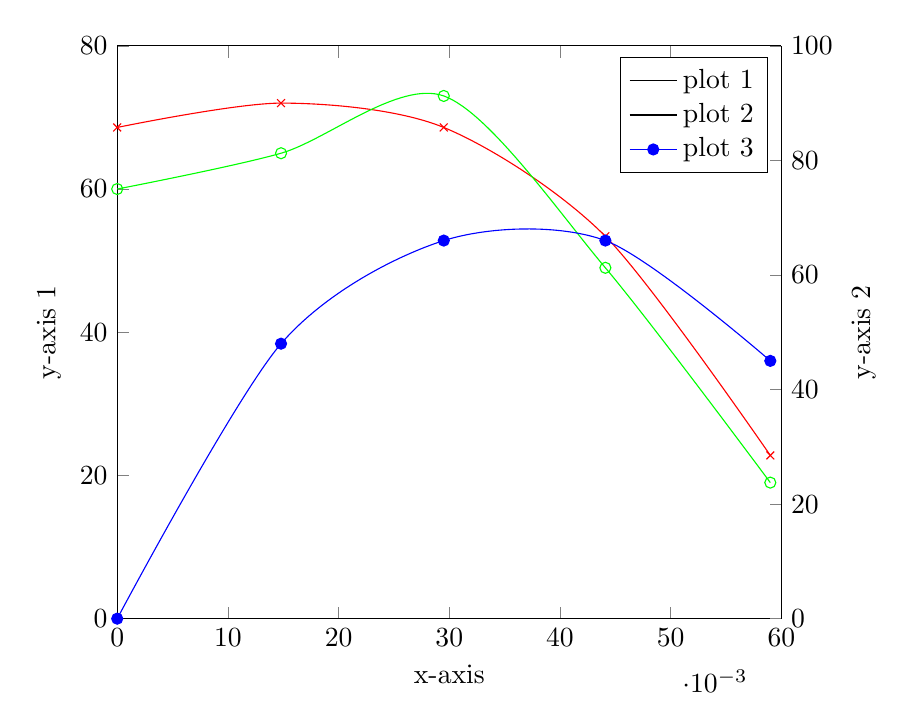
\begin{tikzpicture}
    \pgfplotsset{
        scale only axis,
        scaled x ticks=base 10:3,
        xmin=0, xmax=0.06
    }
    
    \begin{axis}[
      axis y line*=left,
      ymin=0, ymax=80,
      xlabel=x-axis,
      ylabel=y-axis 1,
    ]
    \addplot[smooth,mark=x,red]
      coordinates{
        (0,68.6)
        (0.0148,72)
        (0.0295,68.6)
        (0.0441,53.4)
        (0.059,22.8)
    }; \label{plot_one}
    
    \addplot[smooth,mark=o,green]
      coordinates{
        (0,60)
        (0.0148,65)
        (0.0295,73)
        (0.0441,49)
        (0.059,19)
    }; \label{plot_two}
    
    \end{axis}
    
    \begin{axis}[
      axis y line*=right,
      axis x line=none,
      ymin=0, ymax=100,
      ylabel=y-axis 2
    ]
    \addlegendimage{/pgfplots/refstyle=plot_one}\addlegendentry{plot 1}
    \addlegendimage{/pgfplots/refstyle=plot_two}\addlegendentry{plot 2}
    \addplot[smooth,mark=*,blue]
      coordinates{
        (0,0)
        (0.0148,48)
        (0.0295,66)
        (0.0441,66)
        (0.059,45.0)
    }; \addlegendentry{plot 3}
    \end{axis}
    
    \end{tikzpicture}

由于以上参数是在一米的距离优化的,所以距离更近会导致更多超过临界值的声波。此时表示 \code{0} 的声波可能被误解为表示 \code{1} 的声波,反之亦然。因此丢包率不变但是误码率会增加。

\subsubsection{环境噪声影响}

\begin{table}[h!]
    \centering
    \begin{tabular}{ccc}\toprule
        (cm)& 丢包率 & 误码率 \\\midrule
        \bottomrule
    \end{tabular}
\end{table}

\subsubsection{环境遮挡影响}

\begin{table}[h!]
    \centering
    \begin{tabular}{ccc}\toprule
        障碍物厚度(cm)& 丢包率 & 误码率 \\\midrule
        1 & & \\\midrule
        5 & & \\\midrule
        10 & & \\\midrule
        20 & & \\\midrule
        \bottomrule
    \end{tabular}
\end{table}